\documentclass{report}

\usepackage{biblatex}
\addbibresource{../../Resources/resources.bib}

\usepackage{graphicx}
\usepackage{tikz}
\usetikzlibrary{arrows}
\usetikzlibrary{quantikz}

\usepackage[normalem]{ulem}

\usepackage{physics}
\usepackage{amsthm}
\usepackage{amsfonts}

\newtheorem{definition}{Definition}
\newtheorem{theorem}{Theorem}
\newtheorem{problem}{Problem}
\newtheorem{lemma}{Lemma}

\title{Bridging gates over qubits}
\author{Seyed Sajad Kahani \\ 22222815 \\Supervisor: Prof. Dan Browne}
\date{\today}
\begin{document}
\maketitle

\tableofcontents

\begin{abstract}
  
\end{abstract}

\chapter{Introduction}

Quantum computation (QC) is an emerging field that aims to use quantum mechanics to solve problems that are intractable for classical computers. Since the earliest conceptualization of quantum computation~\cite{feynman1986}, it has been believed that quantum computers could revolutionize the way we solve problems, particularly those involving simulating nature. Over time, it has become clear that quantum computers have applications far beyond physical simulations. There are algorithms for search and traversing graphs, solving linear equations~\cite{montanaro2016}, and methods for machine learning and optimization~\cite{jordan2023}.

Despite significant efforts, we are still far from fully utilizing these algorithms. Our current hardware technology has not yet achieved the desired accuracy and number of qubits necessary for quantum computers to outperform classical computers in solving useful problems. The current situation is commonly referred to as the ``noisy intermediate scale quantum'' (NISQ) era~\cite{preskill2018}, characterized by restricted resources, including a limited number of qubits, constrained qubit connectivity, hardware-specific gate sets, and limited circuit depth due to noise \cite{cross2019}.

The restricted qubit resources and excessive noise susceptibility of NISQ devices necessitate optimal compilers to have any hope of useful near-term quantum computation. A huge amount of research has been conducted to tackle different aspects of the compilation problem, including qubit allocation \cite{itoko2019,siraichi2018,paler2019,zhang2021,li2019}, routing \cite{childs,zhou2020,itoko2019,cowtan2019,nash2020,kissinger2019} and gate synthesis \cite{shende2006,vatan2004,tucci2005,vatan2004a,shende2004,khaneja2001}. These aspects are deeply intertwined and one may not distinguish between them, but all of them are in some sense a circuit transformation from a higher-level circuit (with fewer imposed constraints) to a lower-level circuit (with more imposed constraints) \cite{hundt2022}.

% TODO, improve the information in the following paragraph
While the knowledge of classical compilation is adopted and the divergent points (no-cloning \cite{TODO} and reversibility \cite{TODO}) are studied and addressed well, another important distinction has received less attention - the cost of SWAP operations. In classical circuit synthesis, SWAPs simply rearrange wires at negligible cost, compared to two-bit gates. But in the quantum realm, SWAP gates require double entangling \cite{TODO} interactions between qubits, making them the most expensive two-qubit quantum logic gates \cite{TODO}.

Despite extensive research into minimizing the overall number of SWAP operations~\cite{childs, TODO}, there is little work addressing the inherent cost of each SWAP gate. A few recent works have proposed techniques to reduce the cost of SWAP gates, such as embedding SWAPs within other 2-qubit gates in 2QAN compiler~\cite{lao2021}, or optimization of SWAP decompositions into CNOT gates~\cite{kissinger2019,nash2020}. In this work, we aim to address the primary usage of SWAP gates - enabling connectivity between non-adjacent qubits. We analyze the possibility of simplifications for different connectivity cases.

Here we define a problem called bridging that is to find a circuit that applies a two-qubit gate on two non-adjacent qubits. By utilizing the framework of~\cite{kissinger2019} and the extensive literature of network coding \cite{TODO} show that in the classical case, the cost of bridging over $n$ bits is $4n$ to $6n$ (upto a $O(1)$ constant). We also present a circuit that achieves the lower bounds. We then attempt to extend the results to the quantum regime, by presenting a circuit to bridge two-qubit gates with Schmidt number $2$ over $n$ with optimal number of CNOTs.

This advancement will lead to $33\%$ reduction in the cost of the most expensive two-qubit gate in many situations. To demonstrate the practicality of our results, we implement the algorithms and benchmark with application-oriented dataset of circuits.

The rest of this thesis is organized as follows. Chapter~\ref{chap:background} reviews the related works. In Chapter~\ref{chap:discussion}, we present the algorithms and prove their correctness and optimality for the classical and quantum cases. We implement the algorithms and benchmark against state-of-the-art techniques in Chapter~\ref{chap:implementation}. Finally, Chapter~\ref{chap:conclusion} concludes and discusses avenues for future work.

\chapter{Background}\label{chap:background}

We should be concerned with two key findings from the literature review on quantum compilation. First, the way that they broke down the problem and the assumption they made to simplify the problem space and introducing some structure to that. On the other hand, is the alogrithms that they involve techniques from QC, graph theory and more.

Here we try to review both of these aspects to draw a big picture of our notion of quantum compilation and also to review the existing techniques related to our approach.

We will also briefly discuss network coding and classical compilation for the purpose of self-containedness.

\section{Quantum Compilation}

% General-purpose quantum compilers \cite{cross2022,sivarajah2021,qiskit2023,maronese2021}

The term quantum compilation can be referred any process that transforms a higher-level description of a quantum algorithm into a lower-level description~\cite{hundt2022}. Given the current situation in the most of works \cite{TODO}, circuits are the description used and the compilation hence is the process of transforming a general quantum circuit into a circuit that is compatible with a specific hardware. As the problem of finding the most optimal circuit (with respect to a sense of complexity like depth or number of gates) is proven to be NP-hard \cite{TODO}, the main focus of the research is to break down the problem into smaller problems and to develop techniques to reasonably trade-off between the extension of the process and the quality of the solution. This is pretty much the same as the approach that is taken in classical compilation \cite{TODO}.

The breakdown structure still is not well-established and there are many different approaches \cite{} hence we try to sketch a general picture of the problem and the common patterns in the literature. Afterward we use this general picture as a reference for the rest of this thesis. 

To define such picure, we need to the define the circuit transformation as a process that preserves the semantics of the circuit, i.e. the output of the circuit on any input will be the same before and after the transformation, while it changes the circuit in order to follow some constraints or to optimize the circuit for some goal.

Then, any quantum compilation process can be seen as a series of circuit transformations that each of them is either imposing a constraint or optimizing the circuit (an optimization itself could be seen as a soft constraint \cite{}). The main constraints that are imposed on the circuit are coming from the hardware and are listed below:

\begin{itemize}
  \item \textbf{Gate set}: The set of gates physically available in the hardware.
  \item \textbf{Connectivity}: The connectivity between qubits in the hardware topology.
  \item \textbf{Scheduling}: The timing and parallelizability of gate operations.
\end{itemize}
  
And the optimizations with respect to different degrees of freedom (like assigning qubits, or choosing between equivalent subcircuits). Commonly the goals are one of these:

\begin{itemize}
  \item \textbf{Complexity}: The number of gates or the depth of the circuit.
  \item \textbf{Soft constraints}: The soft constraints associated with one of the constraints above, to be done before the hard constraint is imposed.
\end{itemize}

For example, qiskit\texttrademark, defines the compilation (transpilation) process, as a series of six passes \cite{TODO}. That corresponds to our general picture as follows:

\begin{enumerate}
  \item Init - Unrolling custom gates into one- and two-qubit gates (imposing constraint of gate set with an intermediate gate set).
  \item Layout - Maps logical to physical qubits. (Optimization for connectivity constraints)
  \item Routing - Inserts swap gates to satisfy connectivity. (Imposing connectivity constraints)
  \item Translation - Converts to target gate set. (Imposing gate set constraints)
  \item Optimization - Iteratively optimizes until depth limit reached. (Optimization for reducing two-qubit gates)
  \item Scheduling - Hardware-aware scheduling. (Imposing scheduling constraints)
\end{enumerate}

While, the most common order is always to impose connectivity, then gateset and then scheduling constraints \cite{TODO}, there are some exceptions. For example, the work of \cite{wille2020} assumes a different order, and asks all of the constraints to be resloved before the connectivity constraints.

% TODO, review the processes: tket, ...

With this background established, we now dive into details on gate set constraints, connectivity constraints, scheduling constraints, and circuit optimizations techniques for reducing complexity.

\subsection{Gate synthesis}

Imposing the gate set constraints which is known as the gate synthesis, is one of the oldest subroutines in the quantum compilation. The problem here is to decompose a general $n$-qubit gate into a sequence of gates from a universal gate set. It has been proven in the early days of quantum computing that the set of all one-qubit gates (which can be reduced to 2 gates for approximate synthesis \cite{TODO}) with CNOT and TOFFOLI is a choice for universal gate set \cite{barenco1995}. Afterward, the quest for finding the shortest sequence of gates from this universal gate set for a given gate has been a hot topic in the literature \cite{shende2006,vatan2004}.

While there are many other possible choices for universal gate sets \cite{TODO}, and also most of the existing quantum computers need to decompose CNOTs and they are natively using other families of two-qubit gates, such as~\cite{foxen2020}, still, most of the results in the literature are based on the CNOT gate, and it has become a standard for the intermediate representation of quantum circuits, along with the set of one-qubit gates~\cite{zulehner2018,siraichi2018,li2019,zhang2021,zhou2020,itoko2019,murali2019,sivarajah2021}. Although it may be suboptimal for hardware, it is a theoretically well-studied two-qubit gate.

\subsubsection{Hamiltonian Compilation}

\cite{lao2021,campbell2019,childs2021}

The literature on Hamiltonian compilation is currently limited. Even existing compilers have not implemented anything beyond a first-order Suzuki-Trotter decomposition~\cite{sivarajah2021, qiskit2023}. Also, if we consider the Suzuki-Trotter decomposition as a compiler, there are also a few related works that could be considered as a part of the literature, such as an analysis of its error~\cite{childs2021}.

Not all efforts in Hamiltonian compilation are based on the Suzuki-Trotter decomposition. Another approach is to use a randomized compiler based on sampling Hamiltonian terms~\cite{campbell2019}. This method is called QDRIFT protocol and it is briefly described in the theorem below.

\begin{theorem}[QDRIFT Compiler]
  Given $H = \sum_{j=1}^k h_j$ and an oracle that samples the terms of the Hamiltonian by weight $\frac{\norm{h_i}_\infty}{\sum_{j=1}^k \norm{h_j}_\infty}$, by randomly sampling $N$ terms $\eta_1 \dots \eta_N$, then we can define the approximate evolution as
  \begin{equation}
    U(t) = \prod_{i=1}^N e^{it\frac{\eta}{N}\sum_{j=1}^k \norm{h_j}_\infty}
  \end{equation}
  where it asymptotically outperform first-order Suzuki-Trotter decomposition in number of gates at a certain level of error.
\end{theorem}

Our baseline compiler is described in~\cite{lao2021}, which uses the Suzuki-Trotter decomposition and defines routing and scheduling algorithms specifically for Hamiltonian compilation.

The compiler includes two different heuristic search algorithms, one for initial qubit allocation and another for subsequent qubit allocation. The algorithm for subsequent qubit allocation also provides the route (of SWAP gates) for reallocation. This compiler supports all one and two-qubit gates as intermediate gates, which helps simplify the circuit by unifying consecutive two-qubit gates~\cite{lao2021}.



\subsection{Qubit allocation}


The definition of qubit allocation may vary in the literature, but we can roughly define it as below

\begin{problem}[Qubit Allocation]
  Qubit allocation is the problem of assigning physical qubits of a device to logical qubits of a quantum circuit at each time step to minimize the circuit's complexity.
\end{problem}

We can see that this problem is similar to problem \ref{prob:register_allocation}.

While qubit allocation is NP-hard for arbitrary connectivity graphs, this can be shown easily by a reduction from graph isomorphism~\cite{siraichi2018}. However, real-world devices are not arbitrary, and by imposing some restrictions on the connectivity graph, we can solve the problem in polynomial time~\cite{childs}. For example, the problem is solvable in polynomial time for path graphs, complete graphs, tree graphs, and product graphs. These results has already been known for similar classical problems like token swapping and routing via matching~\cite{banerjee2017}.

\begin{problem}[Routing via Matching]
  Given a graph and a set of pebble, each of them at each node, a permutation is given and we need to achive the permutation by moving the pebbles. each move consists of swapping two pebbles at adjacent nodes. The problem is to find the minimum number of moves (a.k.a. routing number).
\end{problem}

For arbitrary connectivity graphs, there have been attempts to solve the problem, which can be feasible for small devices~\cite{siraichi2018}. The most common approach is to use a heuristic~\cite{zhang2021, itoko2019, cowtan2019} together with a search algorithm (such as BFS, $A^*$\cite{zulehner2018}, simulated annealing\cite{zhou2020}, or others\cite{li2019}) to find a reasonable solution.

In most cases, the treatment of the initial mapping and subsequent mappings is different~\cite{zhou2020, li2019}. This is because while subsequent mappings can be seen as a routing problem in the permutation space, the initial mapping is a search to find the best starting point.

Another approach is to use partial permutations, which allows for the use of the same algorithm for both initial mapping and subsequent mappings~\cite{childs, zulehner2018}.

\begin{definition}[Partial Mapping]
  A partial mapping, is a partial injective function from the logical qubits to the physical qubits.
  It means that some of the logical qubits may not be mapped to any physical qubit.
\end{definition}

Current quantum compilers, such as those used in Qiskit\cite{qiskit2023, cross2022, murali2019} and Tket\cite{sivarajah2021}, use even simpler heuristics, while considering the errors of the device, which is not the case for most papers.

\subsection{Routing}

\subsection{Scheduling}

\subsection{Optimizations}

Circuit optimization is often achieved by applying simplification rules to the circuit~\cite{pointing2021}. These simplification rules are usually based on the commutation relations of the gates~\cite{itoko2019}.

Yet, this simplification rules are implemented as a pattern matching, therefore the hidden patterns that can be revealed by another simplification rules will not be found.


TODO:
\begin{itemize}
  \item Papers with a focus on inital mapping \cite{siraichi2018,zhang2021,paler2019}
  \item Papers with a focus on routing problem \cite{childs,zhou2020,itoko2019,cowtan2019}
  \item Ideas to improve SWAP complexity (embedding from 2QAN and CNOT framework from Kissinger) \cite{lao2021}\cite{nash2020,kissinger2019}
  \item \sout{Papers with a focus on decomposition of gates and KAK} (maybe) \cite{tucci2005,vatan2004a}
  \item Papers with a focus on entangling power (maybe) \cite{nielsen2003,berry2002,bennett2002,linowski2020}
  \item A bit from Network coding \cite{ho2008}
\end{itemize}

\section{Previous Version (From Literature Review)}

\subsection{Classical Compilation}
A detailed study of the principles and heritage of classical compilers could be insightful and influential for any research conducted in the quantum compilation area. Rather than focusing on state-of-the-art results in classical compilation, we will focus on well-established principles to share the experience of classical compilers with quantum compilers.

In the context of executing computer programs, there are two main approaches: interpretation and compilation. Interpretation is the process of processing a program at the time of execution. It means that the processor of the program is aware of the input and the execution environment as well. While compilation refers to the process of transforming a program into another representation before the execution time, so the input and environment are not known at the moment~\cite[p. 2]{aho1986}.

For the quantum case, the transformation of programs (that are represented as gates) will be done before the execution, and the situation is quite similar to classical compilation. We can also assume the possibility of quantum interpretation, which is beyond our scope~\cite{gay2009}.

The process of compilation can be divided into three main phases:

\begin{itemize}
  \item \textbf{Parsing}: Using lexical and syntactic analysis, the source code is transformed into an abstract syntax tree (AST).

  \item \textbf{Intermediate Code Generation}: The AST is transformed into an intermediate representation (IR), which is a lower-level representation that is still device-independent. Any device-independent optimization will also take place here.

  \item \textbf{Target Code Generation}: The IR is transformed into the target code, which is the final representation of the program. The target code is device-dependent, and it is the final representation of the program.
\end{itemize}

Because of the common representation of quantum programs, a quantum compiler will never tackle the parsing phase, while the next two phases could be useful as a guideline for a quantum compiler.

Yet, the influence of classical compilers on quantum compilers may not be limited to the breakdown structure of the compilation process. They will also share some similar subproblems that we define as follows.

\begin{problem}[Register Allocation]
  \label{prob:register_allocation}
  Registers are the fastest memory in a computer. However, they are limited in number and size. Therefore, the compiler must decide at each time which variables should be stored in registers and which should be stored in memory.~\cite[pp. 440-444]{allen2001}
\end{problem}

\begin{problem}[Instruction Scheduling]
  There are some degrees of freedom regarding the order of instructions in a program. The compiler must decide which order is best for the program.~\cite[chap. 10]{allen2001}
\end{problem}

\begin{problem}[Code Motion]
  Code motion is the process of moving code to a different location in the program. This process may result in changes in the code snippets that are moved, but it will not change the semantics of the whole program. The compiler can move code to different locations to improve the performance of the program.~\cite[p. 592]{aho1986}
\end{problem}

\subsection{Quantum Computation}

\subsection{Suzuki-Trotter Decomposition}

The Suzuki-Trotter decomposition~\cite{trotter1959, suzuki1991} is one of the most important tools for dealing with Hamiltonians. This decomposition approximates the time evolution of a Hamiltonian with a sequence of time evolutions of simpler Hamiltonians (terms of the first Hamiltonian). The simplest case is called the Lie-Trotter formula, and it is stated as follows.

\begin{theorem}[Lie Trotter Formula]
For any $H = A + B$,
\begin{equation}
  e^{iH} = \lim_{n \to \infty} (e^{iA/n} e^{iB/n})^n.
\end{equation}
\end{theorem}

Generally, the decomposition is stated as follows.
\begin{theorem}[Higher Order Suzuki-Trotter Decomposition]
  For any $H = \sum_{j=1}^k h_j$, we can define a series of approximations called $\tilde{U}_{2p}$ that
  \begin{align}
\tilde{U}_1(t) &= e^{i h_1 t}\dots e^{i h_k t}, \\
\tilde{U}_2(t) &= e^{i h_1 t / 2}\dots e^{i h_k t / 2} e^{i h_k t / 2}\dots e^{i h_1 t / 2}, \\
\tilde{U}_{2p}(t) &= \tilde{U}_{2p - 2}(u_p t)^2 \tilde{U}_{2p- 2}((1 - 4u_p) t) \tilde{U}_{2p - 2}(u_p t)^2,
  \end{align}
  where $u_p = 1/(4 - 4^{1/(2p - 1)})$.

  Then, 
  \begin{equation}
    \norm{e^{iHt} - \tilde{U}_{2p}(t)} \in O(t^{2p + 1}).
  \end{equation}
\end{theorem}

This could be considered the baseline process for the compilation of Hamiltonians.


\section{Special topics on two-qubit gates}

Another important fact about the gate synthesis of two-qubit gate, which is fruitful for many theoretical purposes is KAK (aka Khaneja-Glaser~\cite{khaneja2001} or Kraus-Cirac~\cite{kraus2001}) decomposition.??

In addition to CNOT gates, it is also inevitable to use SWAP gates while allocating and routing the logical qubits through the physical qubits. However, there is another technique that could be used in some scenarios, called bridge gates~\cite{sivarajah2021,itoko2019,shende2006,siraichi2018} or remote CNOTs~\cite{zhou2020, nash2020}, which will be studied in detail in the next section.


\subsubsection{Kraus-Cirac Decomposition}

The Kraus-Cirac decomposition~\cite{kraus2001} helps us create arbitrary two-qubit gates. It states that any two-qubit gate can be created by a Heisenberg model and local gates.

\begin{theorem}[Kraus-Cirac Decomposition]
For any $U \in SU(4)$, there exist $V_1, V_2, V_3, V_4 \in SU(2)$ together with $\alpha, \beta, \gamma \in \mathbb{R}$ such that
\begin{equation}
  U = V_1 \otimes V_2 e^{\alpha X\otimes X + \beta Y\otimes Y + \gamma Z\otimes Z} V_3 \otimes V_4.
  \end{equation}
\end{theorem}

This theorem, together with the basic properties of entanglement power, will also lead to many more results on communication using two-qubit gates~\cite{berry2002} and also the universality and optimality of three CNOTs for two-qubit gates~\cite{vatan2004}.


\subsection{Entanglement Power}

We already know that there are so many measures for the entanglement of a bipartite state, building upon those measures, we can define entanglement power.

Entanglement power is a measure of the ability of a two-qubit gate to create entanglement. It has multiple definitions, such as the maximum amount of ebits that can be created from product states~\cite{shen2018}, or the average amount of them (with respect to a Haar distribution)~\cite{zanardi2000}, or even the number of terms in a Schmidt decomposition (which will be equal to the number of non-zero terms in the Kraus-Cirac decomposition)~\cite{nielsen2003}.

This measure, assigns a number to each gate, and then, by composing gates, the entanglement power could not exceed the summation of the entanglement powers of the gates that are used to create the gate. This fact is used to prove many tight bounds for decomposition of two-qubit gates.

Moreover, these efforts implicitly define a hierarchy of two-qubit gates based on the number of non-zero terms in the interaction. For example, CNOT has one non-zero term while SWAP has three.

To understand the current state of the art in quantum compilation, we will first look at the general compilation problem. 

\subsection{General Quantum Compilation}


\subsubsection{Qubit Allocation}

\subsubsection{Generic Gate Set}
\subsubsection{Routing and Bridging}

The solution to the qubit allocation problem will not necessarily specify the SWAPs that are needed to change the mapping, although some approaches do so~\cite{childs, li2019, zhou2020}. In other cases, we need to use a routing or search algorithm to find the SWAPs that are required to change the mapping~\cite{zulehner2018, sivarajah2021}.

Moreover, bridge gates can be used as an alternative in cases where we need to SWAP back and forth between two qubits. While most papers use only bridge gates for three qubits~\cite{sivarajah2021,itoko2019,shende2006,siraichi2018} (one qubit in between), the general case of bridge gates is also studied~\cite{zhou2020, nash2020}.

\def\qceq{\midstick[3,brackets=none]{=}}

\begin{figure}[h]
  \label{fig:bridge-one-with-swap}
  \centering
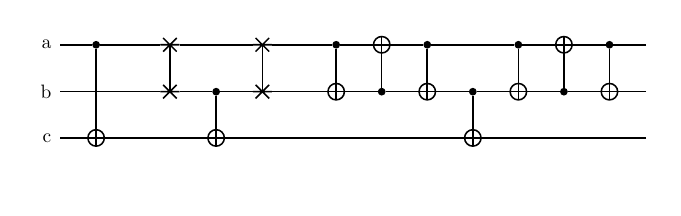
\begin{tikzpicture}
\node[scale=0.7] {
  \begin{quantikz}
  \lstick{a} & \ctrl{2} & \qw \qceq & \swap{1} & \qw & \swap{1} & \qw\qceq & \ctrl{1} & \targ{} & \ctrl{1} & \qw &\ctrl{1} & \targ{} & \ctrl{1} & \qw \\
  \lstick{b} & \qw & \qw & \swap{} & \ctrl{1} & \swap{} & \qw & \targ{} & \ctrl{-1}& \targ{} & \ctrl{1} & \targ{} & \ctrl{-1}& \targ{} & \qw \\
  \lstick{c} & \targ{} & \qw  & \qw & \targ{} & \qw & \qw & \qw & \qw & \qw & \targ & \qw & \qw & \qw & \qw  & \qw \\
  \end{quantikz}
};
\end{tikzpicture}
  \caption{Applying a CNOT gate on $(a, c)$ using a SWAP gate}
\end{figure}

\begin{figure}[h]
  \label{fig:bridge-one-with-bridge}
  \centering
  \begin{quantikz}
  \lstick{a} & \ctrl{2} & \qw \qceq & \qw & \ctrl{1} & \qw & \ctrl{1} & \qw \\
  \lstick{b} & \qw & \qw & \ctrl{1} & \targ{} & \ctrl{1}  & \targ{} & \qw \\
  \lstick{c} & \targ{} & \qw & \targ{} & \qw  & \targ & \qw  & \qw &  \qw \\
  \end{quantikz}
  \caption{Applying a CNOT gate on $(a, c)$ using a bridge gate}
\end{figure}

Figure~\ref{fig:bridge-one-with-swap} and \ref{fig:bridge-one-with-bridge} show the difference between using a SWAP gate and a bridge gate to perform a CNOT gate for the case of three qubits. The bridge gate is more efficient in terms of the number of CNOT gates, but it is less efficient in terms of depth.

Now, the generalized bridge gate is defined as follows~\cite{nash2020}:

\begin{definition}{Generalized Bridge Gate}
  A CNOT between qubit $1$ and $n$ can be performed using a generalized bridge gate as follows:
  \begin{equation} \mathrm{Bridge}(1, n) = \prod_{i=1}^{n - 1}(\mathrm{CNOT}(i + 1, i) \prod_{i=n - 2}^{2}\mathrm{CNOT}(i + 1, i))^2
  \end{equation}
\end{definition}


\def\qceq{\midstick[6,brackets=none]{=}}
\begin{figure}[h]
  \centering
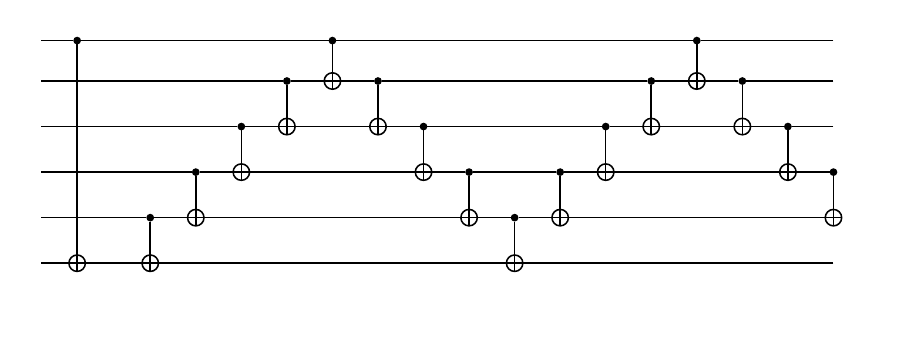
\begin{tikzpicture}
\node[scale=0.7] {
\begin{quantikz}
\qw &\ctrl{5}&\qw\qceq&
 \qw    &\qw     &\qw     &\qw     &\ctrl{1}& \qw    & \qw    & \qw     &
 \qw    &\qw     &\qw     &\qw     &\ctrl{1}& \qw    & \qw    & \qw     & \\
\qw & \qw    & \qw    &
 \qw    &\qw     &\qw     &\ctrl{1}& \targ{}&\ctrl{1}& \qw    & \qw     &
 \qw    &\qw     &\qw     &\ctrl{1}& \targ{}&\ctrl{1}& \qw    & \qw     & \\
\qw & \qw    & \qw    &
 \qw    &\qw     &\ctrl{1}& \targ{}& \qw    &\targ{} &\ctrl{1}& \qw     &
 \qw    &\qw     &\ctrl{1}& \targ{}& \qw    &\targ{} &\ctrl{1}& \qw     & \\
\qw & \qw    & \qw    &
 \qw    &\ctrl{1}&\targ{} & \qw    & \qw    & \qw    &\targ{} &\ctrl{1} &
 \qw    &\ctrl{1}&\targ{} & \qw    & \qw    & \qw    &\targ{} &\ctrl{1} & \\
\qw & \qw    & \qw    &
\ctrl{1}&\targ{} &\qw     & \qw    & \qw    & \qw    & \qw    &\targ{}  &
\ctrl{1}&\targ{} &\qw     & \qw    & \qw    & \qw    & \qw    &\targ{}  & \\
\qw &\targ{} & \qw    &
\targ{} & \qw    & \qw    & \qw    & \qw    & \qw    & \qw     & \qw    &
\targ{} & \qw    & \qw    & \qw    & \qw    & \qw    & \qw     & \qw    & \\
\end{quantikz}
};
\end{tikzpicture}
  \caption{The bridge gate for $n=6$}
\end{figure}

\subsubsection{Circuit Optimization}

\subsection{Hamiltonian Compilation}


\subsubsection{Scheduling}

Even general quantum circuits may have a small degree of freedom in the order of execution. Moreover, the approximate circuit of a Hamiltonian may have a total arbitrariness in the order of execution. This degree of freedom can be set wisely to reduce the complexity of the circuit.

\begin{problem}[Scheduling]
  Given a quantum circuit that has a DAG of dependencies, the scheduling problem seeks for an optimal order of execution of the gates.
\end{problem}

Several heuristic algorithms have been proposed in the literature for both Hamiltonians~\cite{lao2021} and the general case~\cite{zhou2020, zulehner2018}.


\chapter{Discussion}\label{chap:discussion}

While remote gates and ...

It is a well-known fact that a SWAP gate could not be decomposed to less than three CNOTs. For a more complex circuit involving a SWAP or more, this does not necessarily hold in general, especially in presence of connectivity contraints. Here we provide two examples (\ref{ex:swap-swap-decomposition} and \ref{ex:cnot-bridge-decomposition}) with linear connectivity constraints of SWAPs that are used to apply a two-qubit gate on non-adjacent qubits.
They show that decomposing SWAPs to three CNOTs will not necessarily lead to an optimal circuit, even in simple cases.

\begin{figure}[ht]
  \centering
  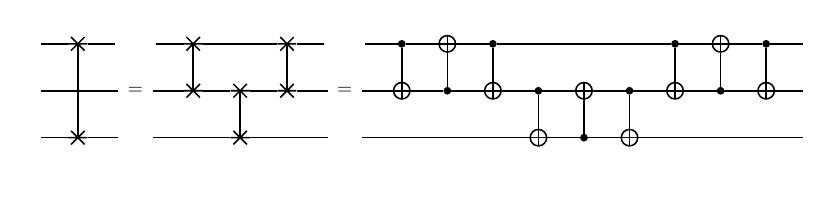
\begin{tikzpicture}
  \node[scale=0.7] {
  \begin{quantikz}
    \qw & \swap{2} & \qw \midstick[3,brackets=none]{=} & \swap{1} & \qw & \swap{1} & \qw \midstick[3,brackets=none]{=} & \ctrl{1}&\targ{}&\ctrl{1} & \qw&\qw&\qw & \ctrl{1}&\targ{}&\ctrl{1} & \qw  \\
    \qw & \qw & \qw & \swap{} & \swap{1} & \swap{} & \qw & \targ{}&\ctrl{-1}&\targ{} & \ctrl{1}&\targ{}&\ctrl{1} & \targ{}&\ctrl{-1}&\targ{} & \qw \\
    \qw & \swap{} & \qw & \qw & \swap{} & \qw & \qw & \qw&\qw&\qw & \targ{}&\ctrl{-1}&\targ{} & \qw&\qw&\qw & \qw \\
  \end{quantikz} };
  \end{tikzpicture} \\

  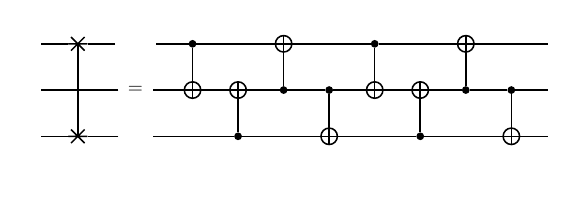
\begin{tikzpicture}
    \node[scale=0.7] {
    \begin{quantikz}
      \qw & \swap{2} & \qw \midstick[3,brackets=none]{=} & \ctrl{1} & \qw &\targ{}& \qw & \ctrl{1}& \qw &\targ & \qw & \qw & \qw \\
      \qw & \qw & \qw & \targ{} & \targ{} & \ctrl{-1} & \ctrl{1} & \targ{} & \targ{} & \ctrl{-1} & \ctrl{1} & \qw \\
      \qw & \swap{} & \qw & \qw & \ctrl{-1} & \qw &\targ{}& \qw & \ctrl{-1}& \qw &\targ & \qw & \qw \\
    \end{quantikz} };
  \end{tikzpicture}
  \caption{Simplifying three SWAP gates}
  \label{ex:swap-swap-decomposition}
\end{figure}

\begin{figure}[ht]
  \centering
  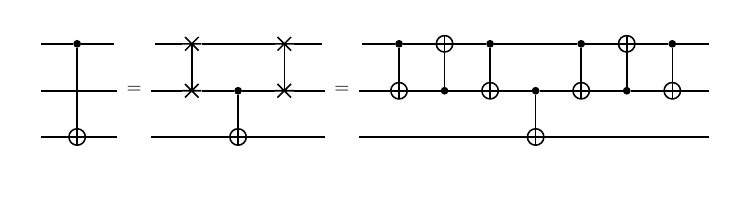
\begin{tikzpicture}
  \node[scale=0.7] {
  \begin{quantikz}
    \qw & \ctrl{2} & \qw \midstick[3,brackets=none]{=} & \swap{1} & \qw & \swap{1} & \qw \midstick[3,brackets=none]{=} & \ctrl{1} & \targ{} & \ctrl{1} & \qw &\ctrl{1} & \targ{} & \ctrl{1} & \qw \\
    \qw & \qw & \qw & \swap{} & \ctrl{1} & \swap{} & \qw & \targ{} & \ctrl{-1}& \targ{} & \ctrl{1} & \targ{} & \ctrl{-1}& \targ{} & \qw \\
    \qw & \targ{} & \qw  & \qw & \targ{} & \qw & \qw & \qw & \qw & \qw & \targ & \qw & \qw & \qw & \qw  & \qw \\
    \end{quantikz}
  };
  \end{tikzpicture} \\
  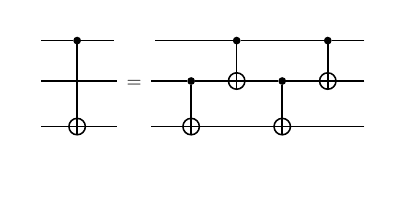
\begin{tikzpicture}
    \node[scale=0.7] {
    \begin{quantikz}
    \qw & \ctrl{2} & \qw \midstick[3,brackets=none]{=} & \qw & \ctrl{1} & \qw & \ctrl{1} & \qw \\
    \qw & \qw & \qw & \ctrl{1} & \targ{} & \ctrl{1}  & \targ{} & \qw \\
    \qw & \targ{} & \qw & \targ{} & \qw  & \targ & \qw  & \qw &  \qw \\
    \end{quantikz}
    };
  \end{tikzpicture}

  \caption{Simplifying a CNOT bridge}
  \label{ex:cnot-bridge-decomposition}
\end{figure}

In order to generalize this idea, we define the following problem

\begin{problem}[Bridging two-qubit gates]
  The solution to the problem of Bridging two-qubit gate $U$ over $n$ qubits is a circuit that can be applied on $n + 2$ qubits such that the $n$ qubits in the middle are not affected and the two qubits on the ends are mapped with respect to $U$. The circuit should normally obey a connectivity and a gate set constraints.
\end{problem}

Note that this definition is valid for classical case as well. In this case, the gate $U$ is a classical reversible gate applying on bits instead of qubits.

% Noting that remote CNOTs and similar things have been already discovered. We will show that the problem of bridging two-qubit gates is a generalization of remote CNOTs and similar things.

\section{Classical Bridging}\label{sec:classical_bridging}

Quantum logical circuits or classical reversible circuits are a class of circuits that are in common between classical and quantum computation. This class has been defined carefuly \cite{shende2003} and it has been proven that any classical reversible circuit can be synthesized using $X$ (classically known as NOT), CNOT and TOFFOLI gates.

Two-bit classical gates are limited to identity, CNOT (in both directions) and SWAP upto local isomorphism (NOT gates).

We will show that CNOT could be bridged over $n$ qubits using $4n + O(1)$ CNOTs within the depth of $2n + O(1)$. Then, we can prove that not only this is result is optimal, but also SWAP has an optimal bound $3n + O(1)$ CNOTs and $3n + O(1)$ depth that is already fulfilled by a simple decomposition.

\begin{theorem}
  Bridging CNOT($a$, $b$) over $n$ bits needs at least $4n$ CNOTs, where $n + 1$ must be the minimum distance between the two bits ($a$, $b$).
  \label{thm:bridging-cnot}
\end{theorem}
\begin{proof}
  We can layer the graph of bits in a way that the first layer is $a$, the last layer is $b$ and there are $n$ layers that we name any bit in layer $i$ as $c_i$. We also define right as the direction towards $b$ and left as th opposite direction.

  By considering a $\mathbb{F}_2$ vector space with hamming inner product $\langle \cdot, \cdot \rangle$ over the bits,  while each bit at each time has a unique vector, we can see that each CNOT as a linear operation adding a vector to another.

  If we name the set of every vector that is associated with a CNOT from layer $i$ to layer $i+1$ with $F_{i\rightarrow i+1}$ and simliarly $F_{i\leftarrow i+1}$, from the fact that the vector $a$ is going to be added to $b$ at the end, we know that the vector $a$ could be extracted from $F_{i\rightarrow i+1}$, which means that $a \in \mathrm{span}(F_{i\rightarrow i+1})$. On the other hand, in order to layer $i$ be unchanged after the process $\sum_{F_{i\leftarrow i+1}} f + \sum_{F_{i-1 \rightarrow i}} f = 0$.
  Mathematically, we can conclude from these two fact that one of these two cases hold for each layer $i$:

  Case 1 ($P(i)$): $F_{i\rightarrow i+1} = D \cup D'$ where $D \cap D' = \emptyset$ and $a \in \mathrm{span}(D)$ and $a \in \mathrm{span}(D')$.

  Case 2 ($Q(i)$): exists $f$ that $\langle f, a\rangle = 1$ and $f \in F_{i+1 \leftarrow i+2}$. 

  We separately prove that for the first case 
  \begin{equation}
    \abs{F_{i \rightarrow i+1}} + \abs{F_{i-1 \leftarrow i}} \geq 4
  \end{equation}
  and for the second case
  \begin{equation}
    \abs{F_{i+1 \rightarrow i+2}} + \abs{F_{i+1 \leftarrow i+2}} \geq 4
  \end{equation}

  Moreover we prove that $P(k+1)$ and $Q(k)$ cannot happen at the same time. This means that if $Q(k)$ holds, $Q(j)$ holds for all $j \geq k$.

  Then assuming $Q(k)$ and $P(k-1)$, by summing up the bounds

  \begin{equation}
    \sum_{i=0}^{k-1} \abs{F_{i \rightarrow i+1}} + \abs{F_{i-1 \leftarrow i}} + \sum_{i=k}^{n-2} \abs{F_{i+1 \rightarrow i+2}} + \abs{F_{i+1 \leftarrow i+2}} \geq 4n - O(1)
  \end{equation}

  This is due to the fact that these two summations has $O(1)$ terms in common. This means that the total number of CNOTs is at least $4n + O(1)$.
\end{proof}

\begin{lemma}[Bound for $P(i)$]
  For the first case used in the proof of Theorem~\ref{thm:bridging-cnot}, we have 
  \begin{equation}
    \abs{F_{i \rightarrow i+1}} + \abs{F_{i-1 \leftarrow i}} \geq 4
  \end{equation}
\end{lemma}
\begin{proof}
  If we call any arbitrary bit in $i$th layer by $c_i$, we know if $a \in F_{i \rightarrow i + 1}$,then it means that there was CNOTs, involving in removing $c_i$ from its site and returning it back. By a simple argument of capacity (in bits) the data could only be stored in the left-hand-side of $i$ meaning that vectors with $c_i$ element appeared in each of $F_{i-1 \leftarrow i}$ $F_{i-1 \rightarrow i}$ twice.

  Now, we already assumed that $a \in \mathrm{span}(D)$ and $a \in \mathrm{span}(D')$. 

  Case 1a: If $a \in D$ or $a \in D'$, then $a \in F_{i \rightarrow {i+1}}$. From the argument above we know that the vectors containing $c_i$ appear twice in $F_{i-1 \leftarrow i}$. One could easily conclude that $\abs{F_{i \rightarrow i+1}} + \abs{F_{i-1 \leftarrow i}} \geq 4$. 

  Case 1b: If $a \notin D$ and $a \notin D'$, then both $D$ and $D'$ need to have two vectors to have $a$ in their span, meaning $\abs{F_{i \rightarrow i+1}} \geq 4$.
\end{proof}

\begin{lemma}[Bound for $Q(i)$]
  For the second case used in the proof of Theorem~\ref{thm:bridging-cnot}, we have 
  \begin{equation}
    \abs{F_{i+1 \rightarrow i+2}} + \abs{F_{i+1 \leftarrow i+2}} \geq 4
  \end{equation}
\end{lemma}
\begin{proof}
  We know that $f \in F_{i+1 \rightarrow i+2}$ that $\langle f, a \rangle = 1$, in addition to that, $
  a \in \mathrm{span}(F_{i \rightarrow i+1})$ and independently $a \in \mathrm{span}(F_{i+1 \leftarrow i+2})$.

  If $\langle f, c_{i+2} \rangle = 0$ it means that $c_{i+2}$ must appear twice in each $F_{i+1 \rightarrow i+2}$ and $F_{i+1 \leftarrow i+2}$, so $F_{i+1 \rightarrow i+2} + F_{i+1 \leftarrow i+2} \geq 4$.

  Otherwise if $\langle f, c_{i+2} \rangle = 1$, then $c_{i+2}$ appears once in $F_{i+1 \leftarrow i+2}$. Noting the order of CNOTs, it must be before CNOTs associated with $a$, therefore all of the terms in $F_{i+1 \rightarrow i+2}$ with $a$ must have $c_{i+2}$ component as well. This makes impossible to $a \in F_{i+1 \rightarrow i+2}$. So $a \in \mathrm{span}(F_{i+1 \rightarrow i+2})$ results in $a$ appears twice, so $\abs{F_{i+1 \rightarrow i+2}} \geq 2$. Putting all together, $\abs{F_{i+1 \rightarrow i+2}} + \abs{F_{i+1 \leftarrow i+2}} \geq 4$.
\end{proof}

It could be easily shown that the circuit that is visualized in Figure \ref{fig:optimal-bridging-cnot} is an optimal solution for bridging CNOT.

\begin{figure}[ht]
  \centering
  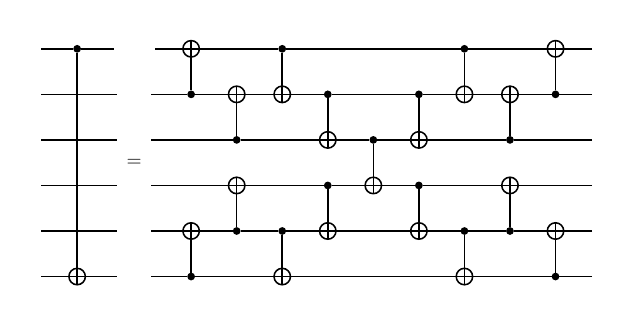
\begin{tikzpicture}
    \node[scale=0.7] {
      \begin{quantikz}
        \qw &\ctrl{5}&\qw \midstick[6,brackets=none]{=} &\targ{}  & \qw     &\ctrl{1}& \qw    & \qw    & \qw    &\ctrl{1}& \qw     &\targ{}&\qw\\
        \qw & \qw    & \qw    &\ctrl{-1}&\targ{}  & \targ{}&\ctrl{1}& \qw    &\ctrl{1}&\targ{} &\targ{}  &\ctrl{-1}&\qw\\
        \qw & \qw    & \qw    & \qw     &\ctrl{-1}& \qw    & \targ{}&\ctrl{1}&\targ{} & \qw    &\ctrl{-1}&\qw & \qw \\
        \qw & \qw    & \qw    & \qw     &\targ{}  & \qw    &\ctrl{1}& \targ{}&\ctrl{1}& \qw    &\targ{}  &\qw & \qw\\
        \qw & \qw    & \qw    &\targ{}  &\ctrl{-1}&\ctrl{1}& \targ{}& \qw    &\targ{} &\ctrl{1}&\ctrl{-1}&\targ{}&\qw \\
        \qw &\targ{} & \qw    &\ctrl{-1}& \qw     & \targ{}& \qw    & \qw    & \qw    &\targ{} & \qw     &\ctrl{-1}& \qw 
        \end{quantikz} };
  \end{tikzpicture}
  \caption{Optimal bridging CNOT}
  \label{fig:optimal-bridging-cnot}
\end{figure}

TODO: Show that two TOFFOLIs (with a NOT in between) are equal to a bridged CNOT over one bit.

TODO: Prove the optimality in presence of TOFFOLI in gate set.

\begin{theorem}
  Bridging SWAP($a$, $b$) over $n$ bits needs at least $6n$ CNOTs, where $n + 1$ must be the minimum distance between the two bits ($a$, $b$).
  \label{thm:bridging-swap}
\end{theorem}
\begin{proof}
  TODO
\end{proof}

\section{Quantum Bridging}

We use a operator propagation framework.

\begin{itemize}
  \item A local opreation does not move the operator.
  \item A $CR_x$ extends operator to two-qubit but doesn't move it (lemmas)
\end{itemize}

\begin{lemma}
  In a two-qubit Hilbert space $\mathcal{H}_A \otimes \mathcal{H}_B$ if $V^{(a)} U^{(a,b)} = U^{(a,b)} V'^{(b)}$ for any $V$, then $U$ has two $CR_x$ gates.
\end{lemma}

\begin{lemma}
  In a two-qubit Hilbert space $\mathcal{H}_A \otimes \mathcal{H}_B$ if $V^{(a)} U^{(a,b)} = U^{(a,b)} V'^{(b)}$ and $V^{(b)} U^{(a,b)} = U^{(a,b)} V'^{(a)}$ each for any $V$, then $U$ has three $CR_x$ gates.
\end{lemma}



TODO: some descriptions and text 

\begin{lemma}
  Any two-qubit gate with Schmidt number $2$ could be written as $L_1 \otimes L_2 CR_x(\theta) L_3 \otimes L_4$ where $L_i$ are local unitaries and $CR_x(\theta)$ is a controlled $R_x$ gate.
  \label{lem:decomposition-schmidt-2}
\end{lemma}
\begin{proof}
  Any two-qubit gate with Schmidt number $2$ could be written as $L_1 \otimes L_2 e^{i\alpha ZZ} L_3 \otimes L_4$. 
  Ignoring the local operations, by applying $R_z(-\theta)$ on the first and the second qubit, we will have 
  \begin{equation}
    R_z(-\theta) \otimes R_z(-\theta) e^{i\alpha ZZ} = CR_z(3\theta)
  \end{equation}
  
  that could be converted to $CR_x(\theta)$ by applying $H$ on the second qubit.
\end{proof}

\begin{theorem}[Optimal bridging For $CR_x$]
  Bridging $CR_x$ over $n$ qubits needs at least $4n$ CNOTs.
  \label{thm:bridging-crx}
\end{theorem}
\begin{proof}
  TODO
\end{proof}

The circuit below, shows how to bridge any two-qubit gate with Schmidt number $2$ over $n$ qubits using $4n$ CNOTs and a $CR_x$.
TODO: the shape (similar to CNOT)

\subsection{Previous Version}

\begin{theorem}[X-shaped bridge]
  Any X-shaped bridge, needs at least $4n$ CNOTs.
\end{theorem}

Proof: As we have already defined the bridge gate for CNOT, we can extend it to any two-qubit gate. Therefore a bridge gate is a circuit consisting of two-qubit gates that acts like $U \in \mathcal{H}^{\otimes 2}$ on the first and last qubits, and the identity on the rest of the qubits.

Note that from a simple argument of light cone, we can conclude that the bridge gate must have two chains of $(1, 2), \dots ,(n-1, n)$ and $(n-1, n), \dots, (1, 2)$ gates.

This two chain may intercept (by the definition below) at any qubit between $1$ and $n$, making one of these shapes

\begin{figure}[h]
  \label{fig:intersections}
  \centering
  a)
\begin{quantikz}
  \qw & \qw & \gate[wires=2]{B} & \qw & \qw \\
  \qw & \gate[wires=2]{A} & \qw & \gate[wires=2]{C} & \qw \\
  \qw & \qw & \qw & \qw & \qw
\end{quantikz}
  b)
\begin{quantikz}
  \qw & \gate[wires=2]{A} & \qw & \gate[wires=2]{C} & \qw \\
  \qw & \qw & \gate[wires=2]{B} & \qw & \qw \\
  \qw & \qw & \qw & \qw & \qw
\end{quantikz}
\caption{Possible intersections of two chains of the bridge gate}
\end{figure}

We stick to the case b, and we know that they are equivalent upto changing numbers.

We know that any two-qubit gate (such as $B$) could be decomposed into

\begin{equation}
  B = (L_2 \otimes L_3) (\alpha^{(1)} I_2 I_3 + \alpha^{(2)} X_2 X_3 + \alpha^{(3)} Y_2 Y_3 + \alpha^{(4)} Z_2 Z_3) (L_2' \otimes L_3')
\end{equation}

where $L_i$ and $L_i'$ are local unitaries on the $i$th qubit.

Then, the whole circuit $ABC$ will be equal to 

\begin{equation}
  ABC = \alpha^{(1)} AL_2 (I_1 I_2) L_2' C \otimes L_3 I_3 L'_3 + \alpha^{(2)} AL_2 (I_1 X_2) L_2' C \otimes L_3 X_3 L'_3 + \dots
\end{equation}

And our final goal is to make a bridge that acts like this for all $U_2$s

\begin{equation}
  U_2 ABC = ABC U_2
\end{equation}

By applying $P^{(i)}_3 L_3^\dagger$ and ${L_3'}^\dagger$ from left and right and then applying $\Tr_3$

\begin{equation}
  U_2 \alpha^{(i)} AL_2 (I_1 \otimes P^{(i)}) L_2' C = \alpha^{(i)} AL_2 (I_1 \otimes  P^{(i)}) L_2' C U_2
\end{equation}

Which directly implies

\begin{equation}
  AL_2 (I_1 \otimes P^{(i)}) L_2' C = V^{(i)} \otimes I
\end{equation}

Note that for all $j, k \in \{1, 2, 3\}$
\begin{equation}
  V^{(j)} V^{(0)\dagger} V_{(k)} V^{(0)\dagger} = AL_2 (I_1 \otimes P^{(i)} P^{(j)}) L_2^\dagger A^\dagger = \sum_k i\epsilon_{jkl} V^{(l)}V^{(0)\dagger}
\end{equation}

Here we use a lemma,
\begin{lemma}[Rotated Paulis]
  If $V^{(j)}$s are unitaries that
  \begin{equation}
    V^{(j)} V^{(0)^\dagger} V^{(k)} V^{(0)^\dagger} = \delta_{jk}I + i\epsilon_{jkl} V^{(l)} V^{(0)^\dagger}
  \end{equation}
  then 
  \begin{equation}
    V^{(j)} = U P^{(j)} U^\dagger V^{(0)^\dagger}
  \end{equation}
  that $U$ is a unitary operation and $P^{(j)}$s are Pauli matrices.
\end{lemma}
\begin{proof}
  If we define $Q^{(j)} = V^{(j)} V^{(0)^\dagger}$, then we have shown that $Q^{(j)}$s are hermitian unitaries that $Q^{(0)} = I$ and $Q^{(j)}Q^{(k)} = \delta_{jk}I + i\epsilon_{jkl} Q^{(k)}$, then $Q^{(j)} = U P^{(j)} U^\dagger$ for some $U$.
  Therefore, $V^{(j)} = U P^{(j)} U^\dagger V^{(0)^\dagger}$
\end{proof}


So far we have shown that
\begin{equation}
  AL_2 (I_1 \otimes P^{(i)}) L_2' C = U P^{(i)} U^\dagger V^{(0)^\dagger} \otimes I
\end{equation}

Then, by defining 
\begin{equation}
  \begin{cases} S_{12} = U^\dagger AL_2 \\
    S'_{12} = L_2' C V^{(0)} U
  \end{cases}
\end{equation}

we can say that
\begin{equation}
  S_{12} (I_1 \otimes P^{(i)}) S'_{12} = P^{(i)} \otimes I
\end{equation}


Now, if we define swap-pair set

\begin{definition}[Swap-Pair Set]
  swap-pair set for any unitary operation $U$ is defined as
  \begin{equation}
    \mathrm{SPS}(U) = \{ (X, Y) | X(I \otimes U)Y = U \otimes I \}
  \end{equation}
\end{definition}


\begin{lemma}[Swap-Pair Set for $Z$]
  Any pair that belongs to $\mathrm{SPS}(Z) \cap \mathrm{SPS}(I)$ 
  can be written as $(\mathrm{SWAP} ~ W ~ \mathrm{CV}, \text{h.c.})$ for some single-qubit gate $W$ and a controlled-$V$ gate.
\end{lemma}
\begin{proof}
Note that it is easy to show that $\mathrm{SPS}(I) = \{ (S, S^\dagger) | \forall S \}$ and 
Also, we can show that if $(S, S^\dagger) \in \mathrm{SPS}(Z)$

\begin{equation}
  \begin{aligned}
  &S(I \otimes Z) = (Z \otimes I) S \\
  \rightarrow &\begin{cases}
    S\ket{00} = (Z \otimes I) S\ket{00} \\
    - S\ket{01} = (Z \otimes I) S\ket{01} \\
    S\ket{10} = (Z \otimes I) S\ket{10} \\
    - S\ket{11} = (Z \otimes I) S\ket{11}
  \end{cases} \\
  \rightarrow &\begin{cases}
    S\ket{00} = \ket{0}\ket{\psi_{00}} \\
    S\ket{01} = \ket{1}\ket{\psi_{01}} \\
    S\ket{10} = \ket{0}\ket{\psi_{10}} \\
    S\ket{11} = \ket{1}\ket{\psi_{11}}
  \end{cases} \\
  \end{aligned}
\end{equation}

Noting that $\braket{\psi_{00}}{\psi_{10}}$ and $\braket{\psi_{01}}{\psi_{11}}$ are zero, there are these two maps then

\begin{equation}
  \begin{cases}
  W\ket{\psi_{00}} = \ket{0} \\
  W\ket{\psi_{10}} = \ket{1} \\
  WV\ket{\psi_{01}} = \ket{0} \\
  WV\ket{\psi_{11}} = \ket{1}
  \end{cases}
\end{equation}

Finally, 
\begin{equation}
  S = \mathrm{SWAP}_{1,2} ~ W ~ \mathrm{CV}_{1\to 2}
\end{equation}
\end{proof}

Now, we need to use the lemma to show that $S_{12}$ and $S'_{12}$ are made of $2$ or $3$ CNOTs.
\begin{equation}
  (S, S') \in \mathrm{SPS}(P_i) \forall i
\end{equation}
  
which means that
\begin{equation}
  \begin{cases} U^\dagger AL_2 = \mathrm{SWAP}_{1,2} ~ W ~ \mathrm{CV}_{1\to 2} \\
    L_2' C V^{(0)} U = \mathrm{CV^\dagger}_{1\to 2} ~ W^\dagger ~ \mathrm{SWAP}_{1,2}
  \end{cases}
\end{equation}

which clearly shows that $A$ and $C$ are made of $2$ or $3$ CNOT and have rank $4$.

By induction, we can expand this argument to all of the gates in the circuit, showing th lower bound of $4n$ CNOTs any bridging.


\chapter{Implementation}\label{chap:implementation}

TODO:
\begin{itemize}
  \item Qiskit: implementation in the routing stage \url{https://qiskit.org/documentation/apidoc/transpiler.html#routing-stage}
  \item tket: just test if it can do any of these simplifications
  \item PyZX (can do some of these simplifications)
\end{itemize}

\chapter{Conclusion}\label{chap:conclusion}

TODO

\printbibliography

\end{document}

